\chapter{基于规划反馈的图推理求解方法}
\label{chp:method}

图推理任务要求模型在自然语言描述、图结构表示、算法约束和答案格式之间建立稳定映射。与一般问答任务相比，图推理的中间过程更长，约束更显式，最终答案通常还需要通过程序执行或规则检查进行验证。如果直接令大语言模型一次性生成答案，模型需要同时完成任务理解、算法选择、代码或推理步骤组织以及结果格式化，容易出现任务类型误判、图约束遗漏、API 使用错误和答案格式不一致等问题。针对这些问题，本文提出一种基于规划反馈的图推理求解方法，将图推理过程拆解为结构化解析、规划生成、规划引导检索、程序化执行验证和反馈推理等阶段，使规划结果作为前向约束指导知识检索和候选程序生成，使执行验证结果作为反向反馈修正程序实现，并在必要时触发检索补充或规划重写。

本章侧重介绍方法层面的设计，重点说明规划反馈范式如何定义、规划如何生成并作用于知识检索、程序生成如何与执行验证和反馈推理形成闭环，以及该方法为什么能够降低图推理中的错误传播。该方法关注求解语义和推理机制本身，运行期的调度策略、共享黑板、共享缓存管理和配置约束则构成系统层面的支撑。

\section{研究问题定义}

本节对本文所研究的图推理问题进行统一界定，并说明为何需要采用规划反馈范式组织求解过程。本节将从任务形式化描述、规划反馈闭环以及方法整体流程三个方面给出问题定义，为后续规划生成、知识检索、程序实现和反馈推理等方法展开提供一致的问题背景。

给定自然语言问题 $Q$ 以及与之关联的图数据，图推理任务的目标是输出满足题目语义和格式要求的答案 $A$。其中，图数据可以显式出现在题目文本中，也可以作为结构化输入提供。本文将图表示为
\begin{equation}
G=(V,E,\mathcal{X})
\end{equation}
其中 $V$ 表示节点集合，$E$ 表示边集合，$\mathcal{X}$ 表示与节点、边或全局图相关的附加属性，例如边权、方向、容量、时间戳、标签和约束参数等。对于动态图任务，$\mathcal{X}$ 还可包含事件序列或时间窗口；对于组合优化任务，$\mathcal{X}$ 则可能包含必须访问、互斥、容量或目标函数等约束。

为了统一不同基准测试集中的任务形式，本文将自然语言问题解析为结构化任务描述
\begin{equation}
T=(\tau,\mathcal{C},\mathcal{O},\mathcal{F})
\end{equation}
其中 $\tau$ 表示任务类型，如最短路径、最大流、匹配、旅行商、拓扑排序或动态图查询；$\mathcal{C}$ 表示任务约束集合，如起点终点、是否带权、是否有向、是否必须回路、是否要求最优性等；$\mathcal{O}$ 表示目标函数或判定目标；$\mathcal{F}$ 表示输出格式要求。于是图推理任务可以写作
\begin{equation}
A=\mathrm{Solve}(Q,G,T)
\end{equation}
即系统需要在理解 $Q$ 与 $G$ 的基础上，依据任务描述 $T$ 生成最终答案。

下文统一使用 $Q$ 表示原始自然语言问题，$G$ 表示规范化后的图数据，$T$ 表示结构化任务描述，$P$ 表示规划结果，$K$ 表示检索得到的知识集合，$C$ 表示候选程序，$F$ 表示执行反馈，$A$ 表示最终答案。

这一形式化定义主要突出图推理中的两点要求。首先，图推理不能只被看作文本理解问题，最终答案需要同时满足图结构约束和算法约束。例如，在路径类任务中，输出的节点序列必须保证相邻节点之间确实存在边；在旅行商问题中，结果不仅要访问所有节点，还需要形成闭合回路，并满足代价优化目标。其次，图推理也不能简单等同于程序执行。原始任务中的目标描述、约束条件和输出格式通常以自然语言给出，系统需要先完成语义解析，才能进一步选择合适的图算法并构造可执行过程。

基于这一认识，本文没有把大语言模型直接作为最终答案生成器，而是将其作为不同智能体的语义理解与推理能力来源。各智能体围绕结构化任务表示、算法规划、外部知识和执行反馈进行协同，使原本难以观察的一次性生成过程，转化为可以逐步检查、定位和修正的多阶段求解过程。

本文所称规划反馈，包含两个方向的约束关系：一是由规划到下游生成的前向约束，二是由执行反馈到上游语义的反向修正。给定结构化任务描述 $T$，规划智能体生成算法级规划
\begin{equation}
P=\{p_1,p_2,\ldots,p_n\}
\end{equation}
其中每个 $p_i$ 对应一个明确的求解动作，例如图构建、候选算法选择、约束检查、结果计算和答案格式化。规划 $P$ 不直接等同于程序代码，而是承担中间语义的作用：它将自然语言问题压缩为可执行求解路线，并为检索和编码提供稳定条件。

在前向求解过程中，规划结果用于约束后续的知识检索和程序生成。检索智能体依据规划 $P$ 召回与当前算法步骤相匹配的外部知识，编码智能体则结合规划 $P$ 和检索知识 $K$ 生成候选程序 $C$。该过程可形式化表示为

\begin{equation}
K=\mathrm{SearchAgent}(P),\quad C=\mathrm{CodingAgent}(P,K)
\end{equation}
与直接使用原始问题文本检索相比，规划查询更接近算法实现语义，能够降低题目叙述噪声对检索结果的干扰；与直接生成程序相比，规划又为代码结构提供了约束，减少模型在控制流、算法选择和约束检查上的随意性。

在反向方向上，执行验证将候选程序的运行状态转化为反馈信号。若程序在测试样例或目标输入上出现语法错误、运行异常、约束违反或格式错误，系统会形成反馈 $F_t$，并据此更新候选程序、检索知识或规划结果：
\begin{equation}
(P_{t+1},K_{t+1},C_{t+1})=\mathrm{Revise}(P_t,K_t,C_t,F_t)
\end{equation}
在大多数情况下，反馈首先用于局部修复候选程序；当错误显示知识条目不匹配时，系统触发补充检索；当错误表明规划遗漏关键约束或任务类型判断错误时，系统才回退到规划阶段。因此，反馈机制并非在报错后直接重新生成，而是先对当前求解状态进行错误归因，再选择相应的修正路径。这里定义的是方法层面的反馈语义，具体的状态记录、事件同步和预算配置由第四章的系统调度机制承担。

这种范式使图推理过程具有更强的可解释性。若最终答案错误，系统能够检查规划是否覆盖任务约束、检索知识是否与规划步骤匹配、候选程序是否通过约束验证，进而将错误定位到相对明确的阶段。相比端到端生成，规划反馈机制不是依赖单次生成质量，而是通过中间表示和外部反馈逐步压缩错误空间。

本文方法的整体流程如图\ref{fig:framework_overview}所示。系统首先由问题智能体对输入问题进行结构化解析，得到任务类型、图结构信息、约束集合和输出格式；随后由规划智能体生成算法级伪代码规划；检索智能体根据规划召回外部图算法知识；编码智能体结合规划与知识生成候选程序；最后由执行验证和反馈推理过程对候选程序进行测试、修正、重生成和答案格式化。

\begin{figure}[htbp]
    \centering
    
\includegraphics[width=\textwidth]{figures/paper/framework.pdf}
    \caption{基于规划反馈的图推理协同求解框架}
    \label{fig:framework_overview}
\end{figure}

图\ref{fig:framework_overview}中的关键不在于简单串联多个智能体，而在于每个阶段都产生可被后续阶段消费的中间语义。问题智能体输出的结构化任务表示降低了原始文本噪声；规划智能体输出的伪代码规划明确了求解路线；检索智能体输出的知识集合补充了 API 和算法细节；编码智能体输出的候选程序将规划转化为可执行对象；执行验证过程输出的反馈信号则为修复和回退提供依据。

从输入和输出形式看，本文方法并不是一个只接收问题文本并直接返回答案的黑盒系统。系统输入由原始问题描述、图结构信息和答案格式约束共同组成；系统输出也不只包含最终答案，还保留结构化任务表示、规划结果、检索知识、候选程序和执行反馈等阶段结果。这些阶段结果对方法分析具有直接作用：一方面，它们可以展示不同阶段如何影响最终求解；另一方面，当系统出现错误时，也可以据此判断问题来自任务解析、规划、检索、编码还是验证环节。

综合来看，本章后续内容主要围绕三条线索展开。第一，规划如何由自然语言任务生成，以及如何判断规划是否覆盖任务目标、算法步骤和关键约束。第二，规划如何进一步引导知识检索，使外部知识调用围绕同一求解语义进行。第三，程序生成如何在执行反馈驱动下完成验证、修复和必要的重生成。上述三条线索分别对应前向规划约束、知识增强支撑和反向反馈修正，共同构成本文方法区别于直接推理方法和一般检索增强生成方法的核心。

\section{基于结构化任务的规划生成方法}

规划生成是本文方法的核心起点。对于图推理任务而言，规划并不是一般意义上的思维链描述，而是从自然语言问题到可执行程序之间的中间求解语义。本节从任务结构化解析、伪代码规划生成、规划表示设计以及规划质量评价四个方面说明规划生成方法。

\subsection{任务结构化解析}

问题智能体负责从原始输入中抽取任务目标、图结构和答案格式约束，其过程可形式化为
\begin{equation}
(T,G) \leftarrow \mathrm{QuestionAgent}(Q)
\end{equation}
其中，$T$ 为结构化任务描述，$G$ 为图数据表示。对于输入中已经显式给出边列表或邻接矩阵的样例，问题智能体主要负责规范化节点、边、权重和方向；对于输入中以自然语言描述图关系的样例，问题智能体还需要将文本中的关系转换为可计算的图结构。

任务结构化解析包含四类信息。第一类是图结构属性，包括图是否有向、是否带权、是否含容量或时间属性、是否存在多重边等。第二类是任务目标，如求最短路径、判断连通性、寻找最大流、计算匹配、寻找团结构或求解组合优化目标。第三类是约束条件，如起点和终点、必须访问的节点、是否要求闭合回路、是否允许重复节点、是否只考虑某个时间窗口等。第四类是输出格式，如返回数值、路径序列、布尔值、节点集合或自然语言解释。

结构化解析并不直接承担求解任务，它的主要作用是为后续规划生成提供稳定、明确的输入。若任务类型或关键约束在这一阶段没有被显式提取，规划结果就可能从一开始偏离正确方向。例如，对于旅行商问题，若解析阶段没有识别回到起点这一约束，规划阶段可能只生成一条覆盖所有节点的路径，而不是闭合回路；在最大流问题中，若容量字段未被识别，程序生成阶段可能将边权误用为普通距离。由此可见，解析阶段对约束的保真度直接影响规划质量。

\subsection{伪代码规划生成}

规划智能体基于结构化任务描述生成算法级伪代码规划：
\begin{equation}
P \leftarrow \mathrm{PlanningAgent}(T)
\end{equation}
其中 $P=\{p_1,p_2,\ldots,p_n\}$ 表示一系列求解步骤，每个步骤对应一个清晰的算法动作。本文采用伪代码而不是自然语言长段解释，主要是为了让规划同时服务于知识检索、程序生成和执行验证。伪代码不要求完全符合某种编程语言语法，但需要明确输入、计算、约束检查和输出之间的关系。

以带权最短路径任务为例，规划通常包含构建带权图、读取源点和目标点、调用最短路径算法、计算路径总代价、按要求格式化输出等步骤。对于旅行商问题，规划则包含构建带权无向图、固定起点或选择起点、枚举或搜索满足哈密顿回路约束的候选路径、计算每条回路总代价、返回最小代价路径等步骤。不同任务的规划内容不同，但都遵循图构建—算法执行—约束验证—结果整理的基本结构。

为了避免规划成为不可执行的自由文本，本文在生成阶段引入三类约束。首先，规划需要显式指明任务族和核心算法方向，避免后续检索在过宽范围内搜索。其次，规划需要单独列出关键约束，而不是把约束隐含在泛化描述中。最后，规划步骤需要保持合理顺序，尤其要避免先进行结果格式化、再补充图构建或约束检查这类顺序错误。通过这些约束，规划能够承担前向骨架的作用，为下游检索、编码和验证提供稳定语义。

\subsection{规划表示设计}

本文对规划表示提出三个设计要求。第一，原子性。每条规划步骤应尽量只表达一个核心动作，避免一条语句中混合构图、算法调用和输出整理等多个目标。原子化步骤有利于后续将规划映射为检索查询、程序片段和验证检查点。第二，约束显式性。对于起点固定、必须回路、容量限制、时间过滤、节点不重复等关键约束，规划需要以独立步骤或标签形式给出。第三，工具无关性。规划本身不绑定某个具体库函数名，而是描述算法语义；具体 API 选择交由检索和编码阶段完成。

在这种表示方式下，规划不是单纯的自然语言说明，也不是可以直接运行的完整代码，而是位于任务语义和程序实现之间的一层中间表示。它保留了一定抽象性，因此可以适配不同的图计算库和执行环境；同时又明确给出算法步骤和关键约束，能够对后续检索和编码形成约束。与自由形式的思维链相比，规划表示减少了冗余解释和随机展开；与直接生成代码相比，它又能更清楚地保留任务目标和算法意图。

需要说明的是，规划阶段本身也可能出错。根据实验中的错误情况，常见问题包括任务类型判断错误、关键约束遗漏、步骤描述过粗、步骤顺序不合适以及算法选择方向偏差等。任务类型判断错误会使后续检索和代码生成从一开始偏离目标；约束遗漏可能导致程序虽然能够运行，但输出结果并不符合题意；步骤描述过粗会使编码智能体缺少必要的实现依据；步骤顺序不合适则可能使生成程序的控制流程变得混乱。本文并不默认规划结果一定正确，而是利用执行反馈对规划进行间接检查。当错误信息多次指向同一类约束缺失或算法偏差时，系统可以回退到规划阶段，对原有规划进行修正。

\subsection{规划质量评价指标}

为了避免规划质量只停留在主观判断层面，本文定义一组可操作的规划评价指标。设规划结果为 $P=\{p_1,\ldots,p_n\}$，任务真实约束集合为 $\mathcal{C}$，从规划中抽取到的约束集合为 $\mathcal{C}_P$。首先，约束覆盖率定义为
\begin{equation}
\mathrm{Cov}(P)=\frac{|\mathcal{C}_P\cap\mathcal{C}|}{|\mathcal{C}|}
\end{equation}
用于衡量规划是否显式包含题目中的关键约束。覆盖率越高，说明规划越能保留任务边界条件。

其次，步骤一致性用于衡量规划内部是否存在逻辑冲突，记为 $\mathrm{Con}(P)$。例如，若规划前一步声明构建无向图，后一步却按有向图处理边；或者前一步要求寻找最短路径，后一步却按最大流进行输出，则说明规划内部存在不一致。该指标可结合规则检查和轻量语义匹配获得。

再次，可执行性评分用于评估规划是否能够稳定映射为程序骨架，记为 $\mathrm{Exe}(P)$。本文将规划中的动作词映射为标准操作集合，如构图、算法调用、候选枚举、约束校验、结果格式化等。若规划缺少核心动作，或动作顺序与数据依赖关系冲突，则可执行性评分下降。综合三项指标，规划质量总分可表示为
\begin{equation}
\mathrm{Score}(P)=\alpha\,\mathrm{Cov}(P)+\beta\,\mathrm{Con}(P)+\gamma\,\mathrm{Exe}(P)
\end{equation}
其中 $\alpha+\beta+\gamma=1$。

该评分具有两方面作用。在离线分析中，它帮助解释不同样例的失败来源。例如，某些样例并非编码能力不足，而是规划覆盖率偏低，导致后续链路从一开始就缺少关键约束。在运行过程中，它也可以作为回退触发信号：当 $\mathrm{Score}(P)$ 低于阈值时，方法流程优先请求规划重写，而不是直接进入代码生成。这样，规划质量评价成为连接方法设计和反馈修正的重要桥梁。

\section{基于伪代码规划的知识检索方法}

规划生成之后，系统需要先获得与当前求解语义相匹配的外部知识支撑。对于图推理任务而言，外部知识的作用不仅是补充背景事实，更重要的是提供稳定的图算法接口、参数含义和返回格式说明。本节介绍如何构建图算法知识库，如何利用规划引导检索，以及如何对检索结果进行重排序、质量评估与纠偏筛选。

\subsection{图算法知识库构建}

为降低模型仅依赖参数记忆导致的实现不稳定，本文构建了面向图计算的外部知识库。知识库条目主要来自图算法库文档、常见任务说明和接口示例。每个知识条目可表示为
\begin{equation}
k_i=\{name_i, desc_i, input_i, output_i, example_i, tag_i, strip_i\}
\end{equation}
其中 $name_i$ 表示函数或算法名称，$desc_i$ 表示功能描述，$input_i$ 和 $output_i$ 分别表示参数与返回值说明，$example_i$ 表示简要调用示例，$tag_i$ 表示任务类型、图属性和适用约束标签，$strip_i$ 表示从原始条目中拆分出的细粒度知识片段。这里的知识片段主要围绕适用图类型、关键参数含义、返回结果结构、约束检查要点等信息组织，使检索阶段不必将整段文档原样送入编码阶段，而可以按规划步骤重新组合更紧凑的实现依据。

知识库覆盖了多类常见图算法与图任务，包括最短路径、连通性判定、最小生成树、最大流、匹配、拓扑排序、团与独立集、旅行商问题以及部分动态图处理方法。对于已经较为成熟的算法，知识条目主要记录可调用 API、输入参数格式和返回结果结构；对于组合优化类任务，知识条目还会补充可行解检查方法和目标函数计算方式。所有知识条目在向量化后写入检索索引，同时保留任务标签和算法标签，用于后续候选结果的过滤与重排序。

需要说明的是，知识库并不承担替代规划的作用。知识库提供的是实现依据、API 选择线索和约束检查信息，而规划负责确定当前任务应采用的求解思路和步骤顺序。如果直接使用原始问题进行检索，返回结果容易受到背景叙述、输出格式说明或冗余自然语言表达的影响；如果只有规划而缺少知识库支撑，代码生成阶段又可能出现函数选择不当、参数误用或返回值理解错误等问题。因此，本文将规划与知识库设计为相互补充的两个环节：规划明确“应该如何求解”，知识库补充“应当调用什么以及如何实现”。

\subsection{规划引导检索的查询构造}

与直接使用问题文本进行检索不同，本文以规划 $P$ 作为核心查询依据，并结合结构化任务描述中的图属性和约束标签构造检索查询。检索过程可表示为
\begin{equation}
K=\mathrm{SearchAgent}(P,T)
\end{equation}
其中 $K=\{k_1,k_2,\ldots,k_m\}$ 为返回的知识集合。

规划引导检索的第一步是从规划中抽取任务类型、关键动作和约束条件。例如，构建带权无向图并计算从源点到终点的最短路径会被拆解为 weighted graph、shortest path、source target、path length 等检索要素；旅行商规划中的枚举哈密顿回路并最小化总代价则会转化为 traveling salesman、Hamiltonian cycle、cycle cost、minimum route 等检索要素。第二步是结合图属性补充查询标签，如 directed、weighted、capacity、temporal 等。第三步是将上述要素组合为更接近文档表达的检索文本。

这种查询构造策略的本质是语义压缩。自然语言问题中可能包含故事背景、变量解释和输出说明，但真正决定 API 选择的是任务类型、图属性和算法动作。通过规划压缩，检索器更容易命中与实现相关的知识条目。第\ref{chp:system}章中的检索质量实验将验证，不同查询表达方式在 Hit@k 和 MRR 指标上存在明显差异，规划查询能够显著改善知识命中效果。

\subsection{知识重排序、质量评估与纠偏筛选}

检索得到候选知识后，系统还需要结合规划进行重排序和筛选。设候选知识条目为 $k_i$，其语义向量相似度为 $s_{\mathrm{sem}}(P,k_i)$，标签匹配得分为 $s_{\mathrm{tag}}(T,k_i)$，约束一致性得分为 $s_{\mathrm{cons}}(P,k_i)$，则综合得分可表示为
\begin{equation}
s(P,T,k_i)=\lambda_1 s_{\mathrm{sem}}(P,k_i)+\lambda_2 s_{\mathrm{tag}}(T,k_i)+\lambda_3 s_{\mathrm{cons}}(P,k_i)
\end{equation}
其中 $\lambda_1+\lambda_2+\lambda_3=1$。

语义相似度用于衡量知识条目与规划文本的整体相关性；标签匹配用于判断知识条目是否适用于当前图属性和任务族；约束一致性则用于排除可能导致实现偏差的条目。例如，若任务明确要求有向图上的最短路径，则无向图专用或忽略方向的说明应被降权；若任务涉及容量约束，则普通边权路径算法不能被误作为最大流算法；若任务要求返回节点集合，则只返回数值目标的接口说明需要额外补充格式化逻辑。

仅有重排序还不够。对于图推理任务，如果检索结果与规划步骤只存在表面语义相似，而未覆盖关键约束或返回结构，编码阶段仍可能在 API 选择和参数组织上出现偏差。为此，本文引入检索质量评估机制，对候选知识集合是否足以支撑当前规划进行显式判断。为避免与前述排序权重混淆，质量评估阶段使用 $\mu$ 表示各评价项权重。设规划共有 $|P|$ 个关键步骤，其中被候选知识覆盖的步骤比例为 $\mathrm{Cov}_{\mathrm{step}}(K,P)$，关键约束覆盖比例为 $\mathrm{Cov}_{\mathrm{cons}}(K,P)$，候选知识之间的冗余度为 $\mathrm{Red}(K)$，则检索质量得分定义为
\begin{equation}
\mathrm{RQ}(K|P,T)=\mu_1 \max_{k_i \in K} s(P,T,k_i)+\mu_2 \mathrm{Cov}_{\mathrm{step}}(K,P)+\mu_3 \mathrm{Cov}_{\mathrm{cons}}(K,P)-\mu_4 \mathrm{Red}(K)
\end{equation}
其中 $\mu_1+\mu_2+\mu_3+\mu_4=1$。该得分不仅衡量最高相关条目的质量，还同时考虑规划步骤是否被充分支撑、约束信息是否完整以及候选上下文是否存在明显噪声。

在此基础上，系统按照检索质量得分选择不同纠偏动作。本文将低置信度阈值和高置信度阈值分别设为 $\tau_l=0.45$ 和 $\tau_h=0.70$，并在实验中保持固定；该设置用于区分明显不足、基本可用和高置信度三类检索状态。若 $\mathrm{RQ}(K|P,T)\ge \tau_h$，说明当前知识集合已具备较高支撑性，系统直接进入编码阶段；若 $\tau_l \le \mathrm{RQ}(K|P,T)<\tau_h$，系统对候选知识进行片段级精炼，仅保留与当前规划步骤、图属性和关键约束直接相关的知识片段；若 $\mathrm{RQ}(K|P,T)<\tau_l$，则系统触发补充检索，依据缺失的规划步骤或约束标签重写查询，再执行一次面向局部失败点的定向召回。其决策过程可写为
\begin{equation}
\mathcal{A}_{\mathrm{ret}}=
\begin{cases}
\text{DirectCode}, & \mathrm{RQ}(K|P,T)\ge \tau_h,\\
\text{RefineStrip}(K), & \tau_l \le \mathrm{RQ}(K|P,T)<\tau_h,\\
\text{RewriteQuery}(P,T)\rightarrow \text{SearchAgent}, & \mathrm{RQ}(K|P,T)<\tau_l.
\end{cases}
\end{equation}

这种机制借鉴了纠错式检索增强的思想，但并不依赖开放域网页搜索，而是结合图算法知识库和规划反馈框架完成受控补检索。其作用在于避免系统在低质量检索结果上直接进入代码生成，减少无效上下文对候选程序的污染，并降低后续修复轮数。

\begin{table}[htbp]
\centering
\small
\caption{检索质量评估下的分级纠偏策略}
\label{tab:retrieval_correction}
\renewcommand{\arraystretch}{1.15}
\begin{tabularx}{\textwidth}{
>{\centering\arraybackslash}p{2.0cm}
>{\raggedright\arraybackslash}p{3.1cm}
>{\raggedright\arraybackslash}X
>{\raggedright\arraybackslash}X}
\toprule
质量状态 & 判定依据 & 纠偏动作 & 作用 \\
\midrule
高置信度 &
$\mathrm{RQ}(K|P,T)\ge \tau_h$ &
保留高分条目，进入编码 &
减少额外调用，保持上下文简洁 \\
中置信度 &
$\tau_l \le \mathrm{RQ}(K|P,T)<\tau_h$ &
按规划步骤精炼和重组片段 &
降低冗余，增强知识与步骤一致性 \\
低置信度 &
$\mathrm{RQ}(K|P,T)<\tau_l$ &
重写查询并补充检索 &
避免低质知识进入编码，降低修复成本 \\
\bottomrule
\end{tabularx}
\end{table}

通过重排序、质量评估与纠偏筛选，编码智能体接收到的知识集合更紧凑，也更贴近规划意图。该过程并不是为了召回尽可能多的知识，而是为了减少与当前求解无关甚至相互冲突的上下文。对于大语言模型生成代码而言，过多不相关知识可能反而造成上下文噪声，导致 API 混用或算法选择摇摆。因此，知识筛选不只是检索阶段的附加步骤，而是连接规划约束、知识利用和后续编码效率的重要中间机制。

\section{基于执行反馈的推理验证方法}

规划和检索能够降低生成难度，但并不能保证候选程序一次正确。图推理任务的一个重要优势是许多约束可以被程序化检查，因此本文将候选程序生成视为推理验证闭环中的候选构造环节，并重点讨论执行反馈如何驱动验证、修复和重生成。本节说明规划如何映射为候选程序，验证样例如何构造，错误反馈如何表示，以及反馈如何驱动局部修复、补充检索和有界重生成。

\subsection{规划到程序的映射机制}

在本文方法中，程序生成并不是从原始问题直接到代码的跳跃，而是由规划和知识共同约束。编码智能体根据规划 $P$ 和筛选后的知识集合 $K$ 生成候选程序
\begin{equation}
C_0 \leftarrow \mathrm{CodingAgent}(P,K)
\end{equation}
候选程序通常采用 Python 实现，并优先调用成熟图计算库完成核心算法。编码阶段需要满足两个要求：一是忠实执行规划步骤，二是尽量使用检索知识中提供的接口和参数说明，减少模型凭经验随意实现造成的错误。

为了提高映射稳定性，本文将规划到程序的转换显式建模为两阶段过程。第一阶段是从线性规划到操作图。系统将伪代码步骤 $p_i$ 映射为操作节点 $o_i$，并建立依赖边 $e_{ij}$ 表示数据依赖和执行顺序，形成
\begin{equation}
\mathcal{G}_P=(\mathcal{O},\mathcal{E})
\end{equation}
其中，$\mathcal{O}$ 包含构图、算法调用、候选枚举、约束检查和结果整理等节点类型。操作图能够显式表示哪些步骤必须先执行，哪些步骤可以作为独立检查点，进而降低代码组织混乱的风险。

第二阶段是从操作图到程序骨架。系统为不同类型的操作节点分配相应模板片段，例如图初始化、边权读取、算法调用、异常处理、可行性检查和输出封装，再按照依赖关系组织为候选程序。这样，即使模型在局部实现细节上出现偏差，整体程序结构仍受规划约束，不容易出现严重顺序错误。

此外，本文引入约束绑定机制，将规划中的关键约束绑定到程序中的检查点。例如，哈密顿路径或旅行商任务会在结果检查阶段插入节点覆盖完整、节点不重复、路径闭合和代价与边权一致等检查；最大流任务会绑定容量字段和源汇点约束；动态图任务会绑定时间过滤逻辑。通过约束绑定，规划中的语义不再停留在文字层面，而是转化为程序中的可验证条件。

\subsection{候选程序生成与执行验证}

候选程序 $C_0$ 生成后，系统首先在验证样例上执行程序，而不是立即接受其输出。验证样例可以来自题目中的小规模图，也可以由系统根据任务类型构造，但只用于检查构图、约束满足和输出格式，不使用目标测试样本的标准答案。对于可精确求解的任务，验证样例的参考结果由确定性图算法或规则检查器生成；对于组合优化任务，则重点检查候选解的可行性、目标方向和代价一致性。执行验证关注四类问题：语法或导入错误、运行时异常、图算法 API 使用错误以及任务约束违反。若程序无法运行，说明候选实现尚未达到基本可执行要求；若程序可运行但违反约束，则说明其算法或格式化逻辑仍需修正。

执行验证过程可表示为
\begin{equation}
F_t=\mathrm{ExecuteVerify}(C_t,\mathcal{D}_{val},P)
\end{equation}
其中 $\mathcal{D}_{val}$ 表示验证样例集合，$P$ 用于提供约束检查依据，$F_t$ 表示第 $t$ 轮反馈。与普通单元测试不同，这里的验证不仅检查代码是否报错，也检查程序是否实现了规划意图。例如，路径类任务需要检查相邻节点是否存在边、总代价是否与边权一致；组合优化任务需要检查可行性和目标方向；动态图任务需要检查时间窗口是否被正确应用。

当程序通过验证后，系统再将其作用于目标图数据 $G$，获得计算结果 $R$，并根据题目要求生成最终答案：
\begin{equation}
A \leftarrow \mathrm{FormatAnswer}(R,\mathcal{F})
\end{equation}
格式化阶段将程序输出转换为基准测试集要求的答案形式，例如节点序列、数值、布尔判断、节点集合或自然语言说明。若格式化结果不符合输出约束，系统也会将其视为反馈的一部分，而不是简单地认为推理已经完成。

\subsection{验证样例构造与错误反馈表示}

验证样例的设计会直接影响反馈信息的有效性。如果样例过于简单，候选程序可能顺利通过测试，但在真实目标图上仍然遗漏关键约束；如果样例过于复杂，则会增加执行时间，也不利于快速定位错误。为此，本文采用小规模、强约束、可判定的样例构造原则。具体来说，验证样例的规模控制在较小范围内，以保证执行开销可控；样例内容需要覆盖当前任务中的关键图属性和输出约束；样例答案或约束检查结果则应能够通过规则稳定判断。

不同类型任务对应的验证重点并不相同。对于路径类任务，验证样例主要检查路径是否合法、起点和终点是否一致，以及路径代价计算是否正确；对于最大流任务，样例需要显式包含容量字段、源点和汇点，并检查流量守恒条件；对于匹配任务，样例关注同一节点是否被重复匹配；对于旅行商问题，样例需要检查输出是否形成闭合回路、是否覆盖全部节点以及总代价是否正确；对于动态图任务，样例应包含时间过滤前后答案发生变化的情况。验证样例的 oracle 由确定性图算法、小规模枚举求解或规则检查器生成，只用于检查候选程序的可执行性、约束满足情况和输出格式，不读取目标测试样本的标准答案，也不参与最终结果评分。通过这种设计，验证样例可以更容易暴露规划结果与程序实现之间的不一致，同时降低答案泄漏风险。

当候选程序执行失败时，系统将原始报错、触发样例、约束违反位置和关联规划步骤整理为统一反馈。反馈可表示为
\begin{equation}
F_t=(etype_t,msg_t,case_t,loc_t,rel_t)
\end{equation}
其中 $etype_t$ 表示错误类型，$msg_t$ 表示错误摘要，$case_t$ 表示触发错误的验证样例，$loc_t$ 表示程序或输出中的错误位置，$rel_t$ 表示与错误最相关的规划步骤或约束。标准化反馈的作用在于减少推理智能体重新阅读全部上下文的负担，使其能够聚焦于当前失败原因。

\subsection{局部修复与有界重生成}

获得反馈后，系统优先执行局部修复：
\begin{equation}
C_{t+1}\leftarrow \mathrm{ReasoningAgent}(C_t,F_t,P,K)
\end{equation}
局部修复适用于错误范围较小且规划方向仍可信的情况，例如语法错误、变量名不一致、导入缺失、返回格式错误或单个 API 参数使用错误。由于修复过程仍以原规划和检索知识为约束，它通常能够在保留已有正确结构的基础上调整局部实现。

若反馈显示当前知识不足或 API 选择不匹配，系统会触发补充检索，利用错误类型和关联规划步骤构造二次查询。例如，当最大流任务出现容量字段读取错误时，二次查询会强调 capacity 参数、source、sink 和返回值结构；当最短路径任务出现权重字段误用时，二次查询会强调 weight 参数和路径长度计算。补充检索的目标不是重新开始整个求解，而是为当前失败位置提供更准确的实现知识。

若局部修复达到上限仍无法通过验证，或错误表明当前候选程序结构与规划严重不一致，系统将进行有界重生成：
\begin{equation}
C'_0\leftarrow \mathrm{CodingAgent}(P,K,F_{1:t})
\end{equation}
有界重生成不同于完全重新推理，它仍然保留当前规划、检索知识和历史反馈，只重新生成候选程序。这样既避免了无限修补低质量代码，又防止每次失败都从原始问题开始，导致已经正确的规划信息被丢弃。实际运行中，局部修复轮数、重生成次数和补充检索触发阈值均由统一配置约束，使反馈修复过程保持可控。

\subsection{反馈驱动的求解流程}

综合上述过程，算法\ref{alg:plangraph}给出了本文方法的完整推理流程。该算法体现了规划反馈的基本思想：先通过规划确定求解路线，再通过检索补充实现知识，随后在执行验证中不断根据反馈修复候选程序。当错误反馈表明下游实现问题时，系统进行局部修复；当错误反馈指向知识缺失或规划遗漏时，系统才回退到相应上游阶段。其中，$\mathrm{SearchAndCorrect}$ 表示检索智能体先根据规划构造查询并召回候选知识，再进行质量评估；若质量低于阈值，则执行知识片段精炼、查询重写或补充检索。

\begin{algorithm}[!htbp]
\small
\caption{基于规划反馈的图推理协同求解流程}
\label{alg:plangraph}
\begin{algorithmic}[1]
\Require 自然语言图推理问题 $Q$
\Ensure 最终答案 $A$
\State $(T,G) \gets \mathrm{QuestionAgent}(Q)$
\State $P \gets \mathrm{PlanningAgent}(T)$
\State $K \gets \mathrm{SearchAndCorrect}(P,T)$
\State $C \gets \mathrm{CodingAgent}(P,K)$
\For{$t=1$ to $T_{\max}$}
    \State $F_t \gets \mathrm{ExecuteVerify}(C,\mathcal{D}_{val},P)$
    \If{$F_t$ 表示验证通过}
        \State $R \gets \mathrm{Run}(C,G)$
        \State $A \gets \mathrm{FormatAnswer}(R,\mathcal{F})$
        \State \Return $A$
    \ElsIf{$F_t$ 指向局部实现错误}
        \State $C \gets \mathrm{ReasoningAgent}(C,F_t,P,K)$
    \ElsIf{$F_t$ 指向知识不匹配}
        \State $K \gets \mathrm{SearchAndCorrect}(P,T,F_t)$
        \State $C \gets \mathrm{ReasoningAgent}(C,F_t,P,K)$
    \ElsIf{$F_t$ 指向规划遗漏}
        \State $P \gets \mathrm{PlanningAgent}(T,F_t)$
        \State $K \gets \mathrm{SearchAndCorrect}(P,T)$
        \State $C \gets \mathrm{CodingAgent}(P,K)$
    \EndIf
    \If{局部修复达到上限}
        \State $C \gets \mathrm{CodingAgent}(P,K,F_{1:t})$
    \EndIf
\EndFor
\State \Return 基于当前最优候选的格式化答案或失败标记
\end{algorithmic}
\end{algorithm}

图\ref{fig:artifact_feedback}展示了规划反馈闭环中的关键中间语义及其修正路径。与图\ref{fig:framework_overview}强调整体阶段划分不同，该图突出的是方法层面的前向约束和反向反馈：规划如何同时约束检索与编码，验证反馈又如何根据错误归因分别作用于候选程序、知识检索和规划语义。这些中间结果既是方法推理的依据，也是后续运行期状态管理的基本对象。

\begin{figure}[htbp]
\centering

\includegraphics[width=0.92\textwidth]{figures/paper/fig3_2.pdf}
\caption{规划反馈闭环中的中间语义与修正路径}
\label{fig:artifact_feedback}
\end{figure}

从算法流程和反馈链路看，各角色智能体围绕同一组可共享的中间语义协同工作。规划智能体提供求解骨架，检索智能体补充实现知识，编码智能体产生可执行候选，推理智能体根据执行反馈完成纠偏。反馈信息同时关联规划步骤和候选程序位置：前者用于判断错误是否源于任务语义、算法选择或约束遗漏，后者用于确定候选程序中需要修改的具体区域。当规划语义仍然有效时，系统保留已有规划和检索结果，仅对局部实现进行修正；只有在上游语义不完整或知识不匹配时，才重新规划或补充检索。这种分级反馈方式缩小了单次修正的影响范围，也减少了无关阶段的重复生成。

\section{方法有效性分析}

前述小节从规划生成、知识检索和推理验证三个角度说明了本文方法的具体流程。本节进一步分析该方法为什么能够提升图推理求解质量，并说明任务族适配如何支撑方法在不同图推理场景中的泛化。这里关注的是方法层面的有效性来源，即规划反馈如何压缩搜索空间、隔离错误传播，并把不同任务族纳入统一求解范式。

\subsection{搜索空间压缩与误差隔离分析}

端到端生成方法需要在任务理解—算法选择—程序实现—格式输出的联合空间中一次性搜索，候选空间可近似表示为
\begin{equation}
\Omega_{\mathrm{e2e}}=\Omega_T\times\Omega_A\times\Omega_C\times\Omega_F
\end{equation}
其中 $\Omega_T$ 表示任务理解空间，$\Omega_A$ 表示算法选择空间，$\Omega_C$ 表示程序实现空间，$\Omega_F$ 表示格式化输出空间。由于这些空间相互耦合，任一阶段的偏差都可能直接污染最终答案。

本文方法将联合搜索分解为条件搜索。系统先根据 $Q$ 和 $G$ 获得结构化任务 $T$，再生成规划 $P$，随后在 $P$ 的约束下检索知识和生成程序。该过程可理解为
\begin{equation}
\Omega_{\mathrm{pf}}=\Omega_T \times \Omega_{P|T} \times \Omega_{K|P,T} \times \Omega_{C|P,K} \times \Omega_{F|C}
\end{equation}
其中每个阶段的候选空间都受到前一阶段中间语义的约束。虽然分阶段机制会引入额外调用成本，但它降低了模型在无约束联合空间中随机探索的概率，尤其适合图推理中约束明确、算法结构稳定的任务。

从误差传播角度看，端到端方法的错误通常难以定位。最终答案错误时，很难判断问题出在任务理解、算法选择、实现细节还是输出格式。本文方法通过规划、知识、候选程序和反馈等中间语义将错误局部化：规划错误主要表现为约束覆盖不足或步骤冲突；检索错误主要表现为知识条目不匹配；编码错误主要表现为运行异常或约束断言失败；格式错误则主要表现为最终输出不符合评测要求。由于错误类型在结构上可区分，系统可以采用不同修正策略，而不必每次都完全重启推理。

此外，执行反馈为系统提供了外部可观测信号，使修正过程不必完全依赖模型的自我判断。候选程序能否运行，输出路径是否有效，总代价是否计算一致，节点是否重复使用，容量约束是否被满足，这些问题都可以通过规则检查或验证样例进行判断。对于图推理任务来说，结果可检查是一个重要特点。本文方法正是利用这一特点，将大语言模型的生成能力与程序执行结果的可验证性结合起来。

从多智能体协同角度看，搜索空间压缩也对应着角色职责的明确划分。问题智能体主要从输入中恢复任务语义，规划智能体负责组织求解路线，检索智能体补充实现所需的外部知识，编码智能体和推理智能体则将规划落实为程序，并根据反馈进行修正。如果这些职责全部压缩到一次生成中，模型需要在同一上下文中同时维护任务理解、算法选择、工具调用和输出约束等多个目标，局部生成偏差很容易破坏整体一致性。分阶段协同后，每个智能体只需要处理边界更清楚的子问题，后续阶段也可以检查前一阶段输出是否满足自身输入要求。

这种分解并不表示各阶段彼此独立。相反，规划反馈方法的关键在于显式保留阶段之间的条件依赖和反向校正关系。规划结果会影响检索查询，检索结果会影响程序实现，程序执行反馈又会反过来暴露规划或检索中的问题。由于这些依赖关系被记录下来，系统在出现错误后可以选择局部修复、补充检索或重新规划，而不是每次都无差别地重新生成全部内容。

\subsection{规划模板库设计}

为了使规划生成在不同数据集和任务类型上保持相对一致，本文设计了一个轻量级规划模板库。该模板库并不保存具体问题的标准答案，而是针对不同任务族提供基本的动作骨架，用于约束规划结果至少包含必要的求解环节。根据任务目标和约束形式，本文将常见图推理任务划分为路径类、连通与可达类、匹配与流类、组合优化类以及动态图类。

不同任务族对应的规划重点有所差异。路径类任务通常需要依次处理图构建、起点和终点解析、路径算法调用、路径合法性检查以及代价计算。连通与可达类任务更关注图构建、连通分量计算或遍历过程、目标节点可达性判断以及布尔结果输出。匹配与流类任务需要明确容量约束或配对约束，并进一步完成核心算法调用、可行性检查和目标值输出。组合优化类任务一般包含候选解生成、约束过滤、目标函数计算和最优解选择等步骤。动态图类任务则需要在上述基础上额外处理时间窗口过滤、事件序列更新和时序约束检查。

模板库在使用时采用软约束方式。规划智能体可以根据具体题目补充或调整步骤，但如果规划结果缺少对应任务族中的关键动作，系统会给出质量告警，并要求重新生成规划。这样做可以保留大语言模型处理复杂自然语言问题时的灵活性，同时避免规划结果过于松散。对于长尾任务或表述较复杂的样例，模板库能够提供相对稳定的求解骨架，从而减少关键步骤被遗漏的情况。

模板库也支持组合式调用。当一个任务同时包含多种属性时，例如动态图上的最短路径，或带容量约束的路径选择，系统可以将主任务模板与属性子模板组合起来，生成复合规划。通过这种方式，本文不需要为每一个细分任务单独设计完整模板，也能覆盖更多任务变体，从而提高方法在不同图推理场景中的迁移能力。

从方法角度看，模板库的作用不是把图推理任务写成固定规则系统，而是为大语言模型的生成过程提供结构先验。传统规则系统要求研究者手动覆盖大量任务变体，维护成本较高；完全自由生成则缺少稳定边界，容易遗漏关键约束。本文采用的模板库位于二者之间：它只规定每类任务必须包含的最小动作集合，不限制模型根据题目细节添加额外步骤。因此，模板库既能约束规划的下限，又不会完全牺牲大语言模型处理开放表达的能力。

\subsection{任务族适配策略}

任务族适配的核心是将不同图推理任务映射到统一的规划反馈框架中。对于一个新任务，系统首先识别其任务族和关键约束，再选择或组合规划模板，随后根据规划中的算法动作构造检索查询，并在执行验证阶段生成对应检查规则。适配过程关注的是任务语义，而不是具体基准测试集名称。

需要说明的是，此处的任务适配主要指方法层面的适配过程，即系统如何根据任务语义生成对应的规划、检索条件和验证检查点。与运行期任务适配器的配置、注册和调度不同，方法层适配关注新任务为什么可以被纳入规划反馈范式，以及不同任务族如何共享同一组求解语义。

以最短路径任务为例，系统需要判断图是否带权、是否有向，并识别起点、终点以及输出要求，即返回路径本身还是返回路径长度。规划模板确定后，检索阶段主要召回与最短路径相关的 API 和算法说明，验证阶段则检查路径是否连续、起终点是否正确以及路径代价是否一致。对于最大流任务，适配重点转向容量字段、源点和汇点、流量守恒条件以及最大流值计算。对于旅行商问题，系统则需要重点检查节点是否全部覆盖、结果是否形成闭合回路，以及总代价是否满足优化目标。

这种适配方式体现了本文方法的泛化思路。不同任务并不是共用一段固定提示词，而是共用解析、规划、检索、执行和反馈这一套求解流程，并在任务族层面对规划模板和验证规则进行调整。这样可以减少方法对单一数据集格式的依赖，使其在 GraphArena\cite{tang2025grapharena}、NLGraph\cite{chen2024nlgraph}、GraphWiz\cite{gong2024graphwiz}、GraphInstruct\cite{graphinstruct2024}和 LLM4DyG\cite{llm4dyg2024}等不同基准测试集上保持较一致的运行流程。

在接入新的任务族时，适配过程通常包括三个步骤。第一步是确定任务族标签和关键约束，例如判断任务属于路径、流、匹配、组合优化还是动态图查询，并抽取起终点、容量、时间窗口或覆盖约束等条件。第二步是为该任务族补充最小规划动作，包括构图、候选生成、约束过滤、目标计算和格式化输出等。第三步是定义验证检查点，使执行反馈能够判断候选程序是否真正满足任务语义。当这三类条件能够被明确表示时，新任务就可以进入统一的规划反馈流程，而不需要改变方法主体。

\subsection{方法适用性与泛化性分析}

规划反馈方法的优势主要来自结构化分解和执行验证，但它并不适用于所有情形。对于极简单的图查询，例如只需读取节点度数或判断一条边是否存在的任务，分阶段规划、检索和验证可能带来不必要的调用开销。此时，直接程序生成或简单规则解析已经能够稳定解决问题，完整规划反馈流程的收益相对有限。

对于知识库覆盖不足的长尾算法，规划反馈方法也可能受到限制。规划能够指出需要解决的问题，但若外部知识库缺少对应 API、算法说明或实现示例，检索阶段就无法为编码提供充分支持。此时系统仍可依赖模型内部知识生成程序，但稳定性会下降。因此，知识库覆盖范围和条目质量会影响该方法在长尾任务上的表现。

执行反馈的有效性还取决于任务是否具有可验证条件。最短路径、最大流、匹配、旅行商等任务通常具备明确的可行性或最优性检查，因此适合采用程序执行反馈；而某些需要复杂数学证明、开放式解释或难以自动判定正确性的任务，反馈信号可能不够充分。在这类任务中，系统需要额外引入人工标注、符号验证或更强的判定器。

从时间复杂度和调用成本看，规划反馈方法相比端到端生成引入了额外阶段。设规划、检索、编码和验证的平均开销分别为 $c_p$、$c_r$、$c_c$ 和 $c_v$，平均修复轮数为 $\bar{t}$，则单个样例的近似开销可表示为
\begin{equation}
C_{\mathrm{pf}}\approx c_p+c_r+c_c+\bar{t}(c_v+c_{\mathrm{fix}})
\end{equation}
其中 $c_{\mathrm{fix}}$ 表示单轮修复开销。该开销高于一次性生成，但换来了更强的错误可观测性和可恢复性。因此，本文在第\ref{chp:method}章和第\ref{chp:system}章分别报告方法效果、稳定性和效率指标，以展示方法收益与计算代价之间的关系。

综合来看，规划反馈方法更适用于三类特征同时较为明显的图推理任务：任务具有清晰的结构约束，结果可以通过程序或规则进行验证，并且算法实现本身具有一定复杂度。对于这类任务，规划可以减少求解路线的随机性，检索可以补充 API 和算法实现知识，执行反馈则可以及时暴露程序错误或约束遗漏，避免错误在后续阶段继续累积。对于过于简单，或缺少明确验证标准的任务，是否启用完整的规划反馈流程，则需要结合运行成本和预期收益进行判断。上述分析也为后续实验组织提供了依据：实验不应只观察最终精确匹配率，还需要结合检索质量、修复轮数、运行开销和错误类型，判断规划反馈机制在不同任务条件下是否真正发挥作用。

\section{方法验证}
\label{sec:method_validation}

前述小节从方法角度说明了 PlanGraph 如何通过任务结构化、规划生成、知识检索、程序执行和反馈修复降低图推理错误。为了验证上述机制是否真正改善求解质量，实验分析围绕两个问题展开：第一，规划反馈式方法是否能够在不同图推理任务上带来稳定收益；第二，这种收益主要出现在哪些任务类型和错误场景中。相关结果主要刻画规划、检索和执行验证闭环对任务求解质量的影响。

\subsection{方法验证目标与数据集}

本文选取五个图推理基准测试集进行方法验证，包括 GraphArena\cite{tang2025grapharena}、NLGraph\cite{chen2024nlgraph}和 GraphWiz\cite{gong2024graphwiz}，以及 LLM4DyG\cite{llm4dyg2024}和 GraphInstruct\cite{graphinstruct2024}。这些数据集共同覆盖经典图算法、组合优化、自然语言图任务、动态图查询和指令式图操作等场景，既包含以节点、边和权重为核心输入的抽象图推理问题，也包含以自然语言场景或指令形式描述的实际场景化图推理问题。

对比方法包括 GPT-4o\cite{openai2024gpt4o}直接推理、多智能体图推理方法 GraphTeam\cite{li2024graphteam}以及程序生成式图推理方法 GCoder\cite{zhang2025gcoder}。三者分别代表直接提示推理、多智能体协同和程序生成求解路线，用于比较规划反馈闭环相对于现有图推理方法的效果。

从去除数据集内部重复任务后的任务类别看，GraphArena 包含 10 类任务，NLGraph 包含 8 类任务，GraphWiz 包含 9 类任务，LLM4DyG 包含 9 类任务，GraphInstruct 包含 21 类任务。本文在保持公开任务定义不变的前提下统一评价口径，主实验采用精确匹配率（Exact Match, EM）作为评价指标。任务类别和逐任务结果能够反映规划反馈机制在不同图推理场景中的具体作用。

\subsection{不同任务类别上的方法效果}

为了分析规划反馈机制在哪些任务上发挥作用，本文将多个基准测试集中的任务按照求解目标划分为图结构分析、最短路径、匹配问题、流优化和哈密顿类问题五个类别，并统计不同方法在各类任务上的平均表现，如图\ref{fig:category_accuracy_comparison}所示。

\begin{figure}[htbp]
\centering
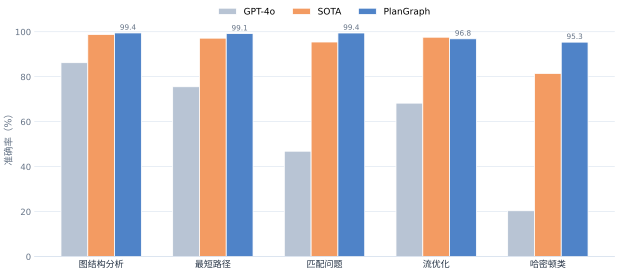
\includegraphics[width=0.94\textwidth]{figures/paper/exp_category_accuracy.pdf}
\caption{不同任务类别上的精确匹配率对比}
\label{fig:category_accuracy_comparison}
\end{figure}

由图\ref{fig:category_accuracy_comparison}可以看出，PlanGraph 在图结构分析、最短路径、匹配问题、流优化和哈密顿类五类任务上均取得了最高精确匹配率。其中，哈密顿类任务的提升幅度最明显。PlanGraph 的平均精确匹配率为 95.33\%，相比最佳现有方法的 74.30\% 高出 21.03 个百分点。该类任务通常同时涉及节点不重复访问、相邻节点连通、回路闭合以及总代价优化等要求。若直接由模型生成答案，容易出现节点遗漏、节点重复访问、路径不可行或代价计算错误等问题。PlanGraph 通过显式规划、程序执行和结果验证，将这些约束转化为可检查的步骤，因此能够更好地减少端到端生成中的结构性错误。

在流优化任务上，PlanGraph 也优于最佳现有方法。具体而言，PlanGraph 在 NLGraph-MF 和 GraphWiz-MF 两个最大流任务中均取得最优结果，两项任务的平均精确匹配率为 96.32\%，相比最佳现有方法的平均结果 94.40\% 提升 1.92 个百分点。最大流任务通常涉及残量图维护、容量更新、反向边处理和增广路径选择等实现细节，对程序实现和 API 使用都有较高要求。PlanGraph 在该类任务上的优势表明，规划生成和外部图算法知识检索能够帮助系统减少最大流求解中的实现偏差。

\subsection{复杂度与样本难度分层分析}

为考察 PlanGraph 在不同计算复杂度任务上的表现，本文将任务划分为 NP 完全任务与非 NP 完全任务两类。按照任务集合中的公开任务定义，本文将邻居查询、距离计算、连通分量和图直径等基础图任务划为非 NP 完全组，将最大独立集、最小点覆盖、最大团、图编辑距离、最大公共子图和旅行商问题划为 NP 完全组。图\ref{fig:np_complete_performance}展示了两类任务上的性能对比。

\begin{figure}[htbp]
\centering
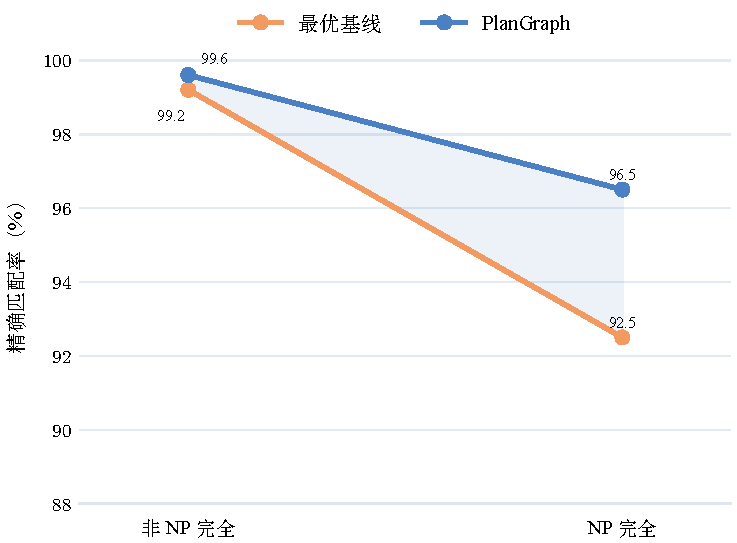
\includegraphics[width=0.86\textwidth]{figures/paper/exp_complexity_trend.pdf}
\caption{NP 完全任务性能对比}
\label{fig:np_complete_performance}
\end{figure}

可以看到，PlanGraph 在非 NP 完全任务上与最佳基线方法均达到 100.00\%，说明基础图任务已经接近饱和，提升空间有限；而在 NP 完全任务上，PlanGraph 的平均精确匹配率达到 96.23\%，较最佳基线方法的 92.87\% 提升 3.36 个百分点，说明规划与验证闭环的主要收益集中体现在高组合复杂度场景。这与最大独立集、最小点覆盖、最大团、图编辑距离、最大公共子图和旅行商问题等任务上的观察一致。

除任务复杂度外，本文还从样本难度角度观察方法表现。该划分以图规模为主要依据：简单样本对应节点数小于 15 的图实例，中等样本对应节点数为 15 至 30 的图实例，困难样本对应节点数大于 30 的图实例。图\ref{fig:sample_difficulty_performance}给出了不同难度样本上的性能对比。

\begin{figure}[htbp]
\centering
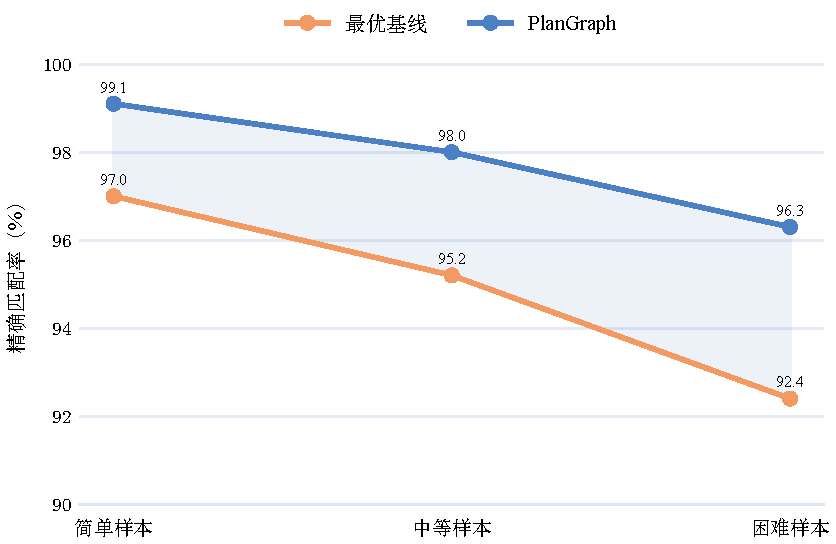
\includegraphics[width=0.86\textwidth]{figures/paper/exp_sample_difficulty_trend.pdf}
\caption{样本难度分层下性能对比}
\label{fig:sample_difficulty_performance}
\end{figure}

从图\ref{fig:sample_difficulty_performance}可见，随着样本难度提高，不同方法的性能均出现下降，但 PlanGraph 的下降幅度相对更小。尤其在困难样本上，PlanGraph 相比最佳基线方法的优势进一步扩大，说明规划先行与执行验证机制对大搜索空间下的稳定求解具有更明显作用。综合两类分层结果可以看出，PlanGraph 的性能收益主要来源于复杂任务场景，而非简单任务上的边际提升。

\subsection{各基准测试集逐任务结果}

为避免总体平均结果掩盖不同任务族之间的性能差异，本文进一步给出五个基准测试集的逐任务精确匹配率统计，以从更细粒度上分析 PlanGraph 在不同图推理场景中的适用性与性能边界。

GraphArena\cite{tang2025grapharena}是面向图计算与图推理任务的综合基准测试集，覆盖邻居查询、连通分量、最短距离、图直径、图编辑距离以及多类组合优化问题。表\ref{tab:grapharena_detail}给出了各方法在该基准测试集各子任务上的逐项结果。其中，CN、CC、SD、GD 和 GED 分别表示邻居查询、连通分量、最短距离、图直径和图编辑距离任务；MIS、MVC、MCP、MCS 和 TSP 分别表示最大独立集、最小点覆盖、最大团、最大公共子图和旅行商问题。

\begin{table}[htbp]
\centering
\caption{GraphArena 各任务精确匹配率（\%）}
\label{tab:grapharena_detail}
\begin{tabular}{lcccc}
\toprule
任务 & GPT-4o & GraphTeam & GCoder & PlanGraph \\
\midrule
CN & \textbf{100.0} & \textbf{100.0} & \textbf{100.0} & \textbf{100.0} \\
CC & \textbf{100.0} & \textbf{100.0} & \textbf{100.0} & \textbf{100.0} \\
SD & \textbf{100.0} & \textbf{100.0} & \textbf{100.0} & \textbf{100.0} \\
GD & \textbf{100.0} & \textbf{100.0} & \textbf{100.0} & \textbf{100.0} \\
GED & 23.3 & 91.0 & 89.5 & \textbf{96.5} \\
MIS & 22.4 & 97.8 & 96.8 & \textbf{98.8} \\
MVC & 19.3 & 98.6 & 97.6 & \textbf{100.0} \\
MCP & 12.5 & 90.5 & 88.7 & \textbf{100.0} \\
MCS & 8.4 & 90.8 & 89.4 & \textbf{95.3} \\
TSP & 4.9 & 82.7 & 80.7 & \textbf{86.8} \\
\bottomrule
\end{tabular}
\end{table}

表\ref{tab:grapharena_detail}显示，基础结构任务对各强基线均已较为简单，CN、CC、SD 和 GD 等子任务几乎都达到满分；图编辑距离和组合优化任务则具有较强区分度。PlanGraph 在这些高约束任务上保持更优结果，说明规划生成、知识检索和执行验证的闭环机制并非只在基础任务的饱和区间内带来边际改善，而是能够更有效地提升复杂图搜索任务中的可行性控制与错误修复能力。

NLGraph\cite{chen2024nlgraph}主要考察自然语言条件下的图算法推理能力，其核心难点不只在于调用某个图算法，而在于先从自然语言描述中恢复图结构、任务目标和求解约束，再完成相应的算法推理。表\ref{tab:nlgraph_detail}给出了各方法在 NLGraph 各子任务上的逐项结果。其中，CONN、MF、CYC、TOPO、SP、BM、HP 和 GNN 分别表示连通性、最大流、环检测、拓扑排序、最短路径、二分图匹配、哈密顿路径和 GNN 推理任务。

\begin{table}[htbp]
\centering
\caption{NLGraph 各任务精确匹配率（\%）}
\label{tab:nlgraph_detail}
\begin{tabular}{lcccc}
\toprule
任务 & GPT-4o & GraphTeam & GCoder & PlanGraph \\
\midrule
CONN & 92.10 & \textbf{100.0} & \textbf{100.0} & \textbf{100.0} \\
MF & 67.30 & 93.67 & 94.10 & \textbf{97.53} \\
CYC & 95.80 & \textbf{100.0} & \textbf{100.0} & \textbf{100.0} \\
TOPO & 60.50 & 91.20 & 92.80 & \textbf{94.80} \\
SP & 72.40 & \textbf{100.0} & \textbf{100.0} & \textbf{100.0} \\
BM & 81.30 & \textbf{100.0} & \textbf{100.0} & \textbf{100.0} \\
HP & 40.70 & \textbf{100.0} & \textbf{100.0} & \textbf{100.0} \\
GNN & 52.10 & 96.80 & \textbf{97.40} & \textbf{97.40} \\
\bottomrule
\end{tabular}
\end{table}

在 NLGraph 上，PlanGraph 对最大流和拓扑排序这类需要算法步骤清晰展开的任务提升更为明显，而在连通性、最短路径、二分匹配和哈密顿路径等已被现有方法较好解决的任务上也至少保持同等水平。该结果说明，PlanGraph 的优势主要体现在把自然语言问题稳定映射到可执行图求解过程这一环节上。

GraphWiz\cite{gong2024graphwiz}是面向指令式图推理场景构建的基准测试集，主要考察模型在给定图操作指令或明确求解要求时，能否完成任务理解、算法选择和结果输出。表\ref{tab:graphwiz_detail}给出了各方法在该基准测试集各子任务上的逐项结果。其中，CONN、CYC、BIP、TOPO、SP、MTS、MF、HP 和 SM 分别表示连通性判定、环检测、二分图判定、拓扑排序、最短路径、最大三角形权重和、最大流、哈密顿路径和子图匹配任务。

\begin{table}[htbp]
\centering
\caption{GraphWiz 各任务精确匹配率（\%）}
\label{tab:graphwiz_detail}
\begin{tabular}{lcccc}
\toprule
任务 & GPT-4o & GraphTeam & GCoder & PlanGraph \\
\midrule
CYC & 95.00 & \textbf{100.0} & \textbf{100.0} & \textbf{100.0} \\
CONN & 70.30 & 86.50 & 90.20 & \textbf{91.20} \\
BIP & 82.70 & 96.30 & 98.00 & \textbf{100.0} \\
TOPO & 75.20 & \textbf{100.0} & \textbf{100.0} & 96.50 \\
SP & 78.60 & 95.00 & 96.40 & \textbf{98.50} \\
MTS & 71.80 & 94.00 & \textbf{95.10} & 93.80 \\
MF & 69.10 & 94.00 & 94.70 & \textbf{95.10} \\
HP & 15.40 & 32.50 & 40.20 & \textbf{99.20} \\
SM & 88.30 & 99.30 & \textbf{99.50} & 98.80 \\
\bottomrule
\end{tabular}
\end{table}

GraphWiz 中差异最明显的是哈密顿路径任务，其对路径约束满足要求极高。PlanGraph 在该任务上远超对比方法，说明显式规划与程序验证对哈密顿路径类问题尤为有效。在连通性判定、最短路径和最大流等需要稳定图构建与步骤执行的任务上，PlanGraph 也保持了较强竞争力。

LLM4DyG\cite{llm4dyg2024}聚焦动态图与时间约束场景，任务通常要求模型同时处理图结构变化、时间顺序以及事件依赖关系。表\ref{tab:llm4dyg_detail}给出了各方法在 LLM4DyG 各子任务上的逐项结果。其中，WL、WC、WTC、WN、WNB、CTC、CTP、FTP 和 SE 分别表示边出现时间查询、首次连通时间查询、三元闭包形成时间查询、给定时间邻居查询、动态图邻居集合查询、三元闭包判定、时序路径判定、时序路径查找和边时间排序任务。

\begin{table}[htbp]
\centering
\small
\caption{LLM4DyG 各任务精确匹配率（\%）}
\label{tab:llm4dyg_detail}
\begin{tabular}{lccccc}
\toprule
任务 & GPT-4o & LLM4DyG & GraphTeam & GCoder & PlanGraph \\
\midrule
WL & 58.00 & 47.30 & 96.33 & 94.33 & \textbf{98.67} \\
WC & 67.33 & 64.10 & 94.33 & \textbf{94.78} & 93.56 \\
WTC & 87.67 & 63.00 & \textbf{100.00} & 97.08 & \textbf{100.00} \\
WN & 33.33 & 45.90 & 95.33 & 94.74 & \textbf{97.47} \\
WNB & 44.67 & 20.00 & \textbf{100.00} & 94.83 & \textbf{100.00} \\
CTC & 77.33 & 66.70 & 99.67 & \textbf{100.00} & 99.33 \\
CTP & 57.67 & 59.80 & 87.00 & \textbf{100.00} & 92.03 \\
FTP & 46.67 & 80.80 & 81.00 & 74.58 & \textbf{84.57} \\
SE & 49.67 & 35.80 & \textbf{99.67} & 93.67 & 99.33 \\
\bottomrule
\end{tabular}
\end{table}

从表\ref{tab:llm4dyg_detail}可以看出，PlanGraph 在边出现时间查询、给定时间邻居查询、动态图邻居集合查询和边时间排序等任务上表现较好，但在首次连通时间查询、三元闭包判定和时序路径判定等任务上尚未全面超过最优对比方法。这说明动态图任务内部差异较大。对于更依赖结构约束检查和过程验证的任务，规划反馈闭环能够带来更明显的收益；而对于需要细粒度时间建模或连续状态跟踪的任务，当前方法仍存在改进空间。

GraphInstruct\cite{graphinstruct2024}面向图指令跟随场景，强调模型能否根据任务指令稳定完成邻居查询、边判断、连通性分析、遍历与拓扑排序等基础图操作。GraphInstruct 原始设置共包含 21 个任务，本文对全部任务进行统计，不对任务集合做抽样或裁剪。表\ref{tab:graphinstruct_detail}给出了各方法在该基准测试集上的逐项结果。其中，NB、BIP、EDGE、CONN、DEG、DFS、PRED、TOPO、CC、CN、HP、JAC、SP、DIAM、PR、MF、MST、BFS、CLUST、CYC 和 EP 分别表示邻居查询、二分图判定、边存在判断、连通性、度数计算、深度优先遍历、前驱查询、拓扑排序、连通分量、公共邻居、哈密顿路径、Jaccard 系数、最短路径、图直径、PageRank、最大流、最小生成树、广度优先遍历、聚类系数、环检测和欧拉路径任务。

\begin{table}[htbp]
\centering
\small
\caption{GraphInstruct 各任务精确匹配率（\%）}
\label{tab:graphinstruct_detail}
\resizebox{\textwidth}{!}{%
\begin{tabular}{lccccc}
\toprule
任务 & GPT-4o & GraphInstruct & GraphTeam & GCoder & PlanGraph \\
\midrule
NB & 98.00 & 99.00 & \textbf{100.00} & 99.53 & \textbf{100.00} \\
BIP & 89.67 & 85.00 & 99.00 & \textbf{100.00} & \textbf{100.00} \\
EDGE & 90.67 & 84.00 & 99.33 & 97.47 & \textbf{100.00} \\
CONN & 92.22 & 83.00 & \textbf{100.00} & \textbf{100.00} & \textbf{100.00} \\
DEG & 98.00 & 81.00 & \textbf{100.00} & 98.67 & \textbf{100.00} \\
DFS & 89.33 & 46.00 & 95.67 & 94.33 & \textbf{96.33} \\
PRED & 47.41 & 41.00 & 98.00 & \textbf{99.75} & \textbf{99.75} \\
TOPO & 59.00 & 33.00 & 98.33 & \textbf{99.50} & 99.25 \\
CC & 39.30 & 83.00 & 94.67 & 83.30 & \textbf{94.74} \\
CN & 49.00 & 23.00 & \textbf{100.00} & 99.53 & 99.69 \\
HP & 33.70 & 18.00 & 97.70 & 98.75 & \textbf{99.16} \\
JAC & 17.00 & 14.00 & \textbf{100.00} & 98.91 & \textbf{100.00} \\
SP & 57.30 & 14.00 & \textbf{100.00} & \textbf{100.00} & 99.44 \\
DIAM & 23.00 & 13.00 & \textbf{100.00} & \textbf{100.00} & \textbf{100.00} \\
PR & 15.30 & 13.00 & 66.43 & 57.01 & \textbf{66.75} \\
MF & 15.00 & 6.00 & 99.30 & 93.67 & \textbf{99.67} \\
MST & 1.00 & 4.00 & 54.86 & 49.19 & \textbf{60.53} \\
BFS & 59.00 & 3.00 & 84.79 & \textbf{94.21} & 93.69 \\
CLUST & 32.00 & 9.00 & 85.06 & 84.93 & \textbf{85.38} \\
CYC & 68.00 & 71.00 & 96.46 & 95.07 & \textbf{97.96} \\
EP & 0.00 & 0.00 & 93.54 & \textbf{100.00} & \textbf{100.00} \\
\bottomrule
\end{tabular}
}
\end{table}

GraphInstruct 主要考察图指令执行能力。PlanGraph 在 21 个任务上的平均精确匹配率为 94.87\%，在 17 个任务上取得最优或并列最优，尤其在邻居查询、二分图判定、连通性、度数计算、PageRank、最小生成树、最大流和欧拉路径等任务上表现稳定，说明所提框架不仅能处理复杂求解型任务，也能处理相对基础但格式要求严格的图查询任务。

\subsection{误差归因}

结合实验过程中的失败样例，当前错误大致可以分为五类，如表\ref{tab:error_taxonomy}所示。这些错误并不只发生在代码实现阶段，也可能从规划、检索、验证或答案格式化阶段逐步累积。因此，图推理任务很难依靠单一模块完全解决，而需要中间表示、外部知识和执行约束共同发挥作用。

\begin{table}[htbp]
\centering
\small
\caption{失败样本的主要错误类型归纳}
\label{tab:error_taxonomy}
\begin{tabular}{m{3cm}m{4.5cm}m{5cm}}
\toprule
错误类型 & 具体表现 & 主要影响阶段 \\
\midrule
任务识别偏差 & 将判定任务误识别为优化任务，或混淆路径搜索与可达性判断 & 规划阶段 \\
约束遗漏 & 忽略固定起点、回路闭合、时间窗口或容量限制 & 规划/编码阶段 \\
API 误用 & 选择语义相近但并不匹配的函数，或参数使用错误 & 检索/编码阶段 \\
边界情况失效 & 在小样例上通过，但在目标图上因特殊结构而失败 & 验证阶段 \\
输出格式错误 & 路径顺序、集合表示或文本格式不符合官方脚本要求 & 答案生成阶段 \\
\bottomrule
\end{tabular}
\end{table}

从整体表现看，PlanGraph 在高约束图任务上已经展现出较强稳定性，但面对动态图、复杂时序逻辑和长尾组合搜索时仍有改进空间。后续可从时序感知规划、失败反馈驱动的知识重排序以及更具代表性的验证样例构造等方面继续完善，以提升方法在更复杂场景下的适用性。


\section{本章小结}

本章围绕基于规划反馈的图推理求解方法进行了说明。该方法先将自然语言形式的图推理任务转换为结构化任务表示，并在此基础上生成算法级伪代码规划；随后，系统利用规划结果约束外部知识检索；最后，在规划和检索知识共同约束下生成候选程序，并通过程序执行和结果检查获得反馈，据此触发局部修复、补充检索或规划重写。相比端到端直接生成答案的方式，该方法通过中间语义表示拆分任务理解、算法选择和程序实现过程，降低了一次性联合生成的难度，同时利用执行反馈及时发现并修正错误，减少错误在后续阶段中的继续传递。

本章还结合五个图推理基准测试集，从任务类别、复杂度分层、样本难度、逐任务结果和误差归因等角度验证了规划反馈式方法的有效性。实验结果表明，该方法的收益主要集中在高约束、强组合和容易出现结构性错误的图推理任务中。下一章将介绍基于黑板调度的多智能体图推理协同框架，说明上述方法如何在系统中完成调度、共享缓存管理、异常恢复和任务扩展。
